\section[Random C. V. Generator]{\textit{Random Control Voltage Generator}}
\sectionmark{\textit{Random C. V. Generator}}
\label{sec:random_generator}



\begin{figure}
	\centering
	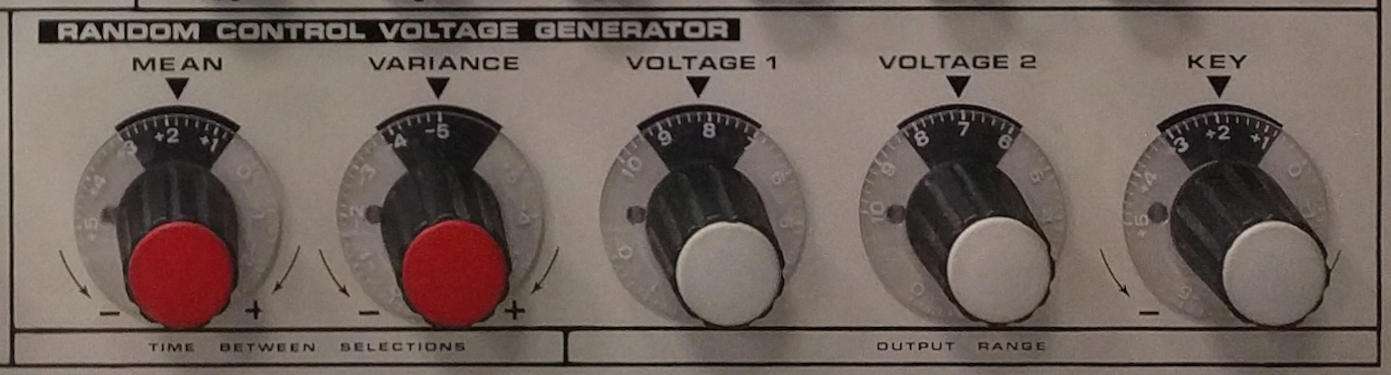
\includegraphics[width=0.7\textwidth]{images/random_generator}
	\caption[\textit{Random Voltage Control Generator}]{Unidad del generador aleatorio de voltaje de control del Synthi 100 del GME, uno de los pocos módulos que no tiene más que una instancia.}
	\label{fig:random_generator}
\end{figure}

\subsection{Implementación en \appName}
Este es el único módulo cuyo generador de señales no está dirigido por una instancia de \texttt{Synth} sino por un \texttt{Routine}. Un \texttt{Synth} es utilizado únicamente para convertir los valores numéricos del \texttt{Routine} a valores de audio y de control. Una <<rutina>> en SuperCollider puede explicarse como una serie de eventos que se suceden uno tras otro y que pueden ejecutarse asíncronamente. Una característica interesante es la posibilidad de situar en el tiempo estos eventos, haciendo esperar a la rutina un número determinado de segundos con el método \texttt{wait(Integer)}. La rutina que gobierna el módulo \textit{Random Control Voltage Generator} se compone de un bucle de valores aleatorios que se suceden con esperas de duración variable. Los valores aleatorios son generados por métodos del propio lenguaje de programación.